% Options for packages loaded elsewhere
\PassOptionsToPackage{unicode}{hyperref}
\PassOptionsToPackage{hyphens}{url}
%
\documentclass[
]{book}
\usepackage{lmodern}
\usepackage{amsmath}
\usepackage{ifxetex,ifluatex}
\ifnum 0\ifxetex 1\fi\ifluatex 1\fi=0 % if pdftex
  \usepackage[T1]{fontenc}
  \usepackage[utf8]{inputenc}
  \usepackage{textcomp} % provide euro and other symbols
  \usepackage{amssymb}
\else % if luatex or xetex
  \usepackage{unicode-math}
  \defaultfontfeatures{Scale=MatchLowercase}
  \defaultfontfeatures[\rmfamily]{Ligatures=TeX,Scale=1}
\fi
% Use upquote if available, for straight quotes in verbatim environments
\IfFileExists{upquote.sty}{\usepackage{upquote}}{}
\IfFileExists{microtype.sty}{% use microtype if available
  \usepackage[]{microtype}
  \UseMicrotypeSet[protrusion]{basicmath} % disable protrusion for tt fonts
}{}
\makeatletter
\@ifundefined{KOMAClassName}{% if non-KOMA class
  \IfFileExists{parskip.sty}{%
    \usepackage{parskip}
  }{% else
    \setlength{\parindent}{0pt}
    \setlength{\parskip}{6pt plus 2pt minus 1pt}}
}{% if KOMA class
  \KOMAoptions{parskip=half}}
\makeatother
\usepackage{xcolor}
\IfFileExists{xurl.sty}{\usepackage{xurl}}{} % add URL line breaks if available
\IfFileExists{bookmark.sty}{\usepackage{bookmark}}{\usepackage{hyperref}}
\hypersetup{
  pdftitle={Reticular Action Model (RAM) Notation},
  pdfauthor={Ivan Jacob Agaloos Pesigan},
  hidelinks,
  pdfcreator={LaTeX via pandoc}}
\urlstyle{same} % disable monospaced font for URLs
\usepackage{color}
\usepackage{fancyvrb}
\newcommand{\VerbBar}{|}
\newcommand{\VERB}{\Verb[commandchars=\\\{\}]}
\DefineVerbatimEnvironment{Highlighting}{Verbatim}{commandchars=\\\{\}}
% Add ',fontsize=\small' for more characters per line
\usepackage{framed}
\definecolor{shadecolor}{RGB}{248,248,248}
\newenvironment{Shaded}{\begin{snugshade}}{\end{snugshade}}
\newcommand{\AlertTok}[1]{\textcolor[rgb]{0.94,0.16,0.16}{#1}}
\newcommand{\AnnotationTok}[1]{\textcolor[rgb]{0.56,0.35,0.01}{\textbf{\textit{#1}}}}
\newcommand{\AttributeTok}[1]{\textcolor[rgb]{0.77,0.63,0.00}{#1}}
\newcommand{\BaseNTok}[1]{\textcolor[rgb]{0.00,0.00,0.81}{#1}}
\newcommand{\BuiltInTok}[1]{#1}
\newcommand{\CharTok}[1]{\textcolor[rgb]{0.31,0.60,0.02}{#1}}
\newcommand{\CommentTok}[1]{\textcolor[rgb]{0.56,0.35,0.01}{\textit{#1}}}
\newcommand{\CommentVarTok}[1]{\textcolor[rgb]{0.56,0.35,0.01}{\textbf{\textit{#1}}}}
\newcommand{\ConstantTok}[1]{\textcolor[rgb]{0.00,0.00,0.00}{#1}}
\newcommand{\ControlFlowTok}[1]{\textcolor[rgb]{0.13,0.29,0.53}{\textbf{#1}}}
\newcommand{\DataTypeTok}[1]{\textcolor[rgb]{0.13,0.29,0.53}{#1}}
\newcommand{\DecValTok}[1]{\textcolor[rgb]{0.00,0.00,0.81}{#1}}
\newcommand{\DocumentationTok}[1]{\textcolor[rgb]{0.56,0.35,0.01}{\textbf{\textit{#1}}}}
\newcommand{\ErrorTok}[1]{\textcolor[rgb]{0.64,0.00,0.00}{\textbf{#1}}}
\newcommand{\ExtensionTok}[1]{#1}
\newcommand{\FloatTok}[1]{\textcolor[rgb]{0.00,0.00,0.81}{#1}}
\newcommand{\FunctionTok}[1]{\textcolor[rgb]{0.00,0.00,0.00}{#1}}
\newcommand{\ImportTok}[1]{#1}
\newcommand{\InformationTok}[1]{\textcolor[rgb]{0.56,0.35,0.01}{\textbf{\textit{#1}}}}
\newcommand{\KeywordTok}[1]{\textcolor[rgb]{0.13,0.29,0.53}{\textbf{#1}}}
\newcommand{\NormalTok}[1]{#1}
\newcommand{\OperatorTok}[1]{\textcolor[rgb]{0.81,0.36,0.00}{\textbf{#1}}}
\newcommand{\OtherTok}[1]{\textcolor[rgb]{0.56,0.35,0.01}{#1}}
\newcommand{\PreprocessorTok}[1]{\textcolor[rgb]{0.56,0.35,0.01}{\textit{#1}}}
\newcommand{\RegionMarkerTok}[1]{#1}
\newcommand{\SpecialCharTok}[1]{\textcolor[rgb]{0.00,0.00,0.00}{#1}}
\newcommand{\SpecialStringTok}[1]{\textcolor[rgb]{0.31,0.60,0.02}{#1}}
\newcommand{\StringTok}[1]{\textcolor[rgb]{0.31,0.60,0.02}{#1}}
\newcommand{\VariableTok}[1]{\textcolor[rgb]{0.00,0.00,0.00}{#1}}
\newcommand{\VerbatimStringTok}[1]{\textcolor[rgb]{0.31,0.60,0.02}{#1}}
\newcommand{\WarningTok}[1]{\textcolor[rgb]{0.56,0.35,0.01}{\textbf{\textit{#1}}}}
\usepackage{longtable,booktabs}
\usepackage{calc} % for calculating minipage widths
% Correct order of tables after \paragraph or \subparagraph
\usepackage{etoolbox}
\makeatletter
\patchcmd\longtable{\par}{\if@noskipsec\mbox{}\fi\par}{}{}
\makeatother
% Allow footnotes in longtable head/foot
\IfFileExists{footnotehyper.sty}{\usepackage{footnotehyper}}{\usepackage{footnote}}
\makesavenoteenv{longtable}
\usepackage{graphicx}
\makeatletter
\def\maxwidth{\ifdim\Gin@nat@width>\linewidth\linewidth\else\Gin@nat@width\fi}
\def\maxheight{\ifdim\Gin@nat@height>\textheight\textheight\else\Gin@nat@height\fi}
\makeatother
% Scale images if necessary, so that they will not overflow the page
% margins by default, and it is still possible to overwrite the defaults
% using explicit options in \includegraphics[width, height, ...]{}
\setkeys{Gin}{width=\maxwidth,height=\maxheight,keepaspectratio}
% Set default figure placement to htbp
\makeatletter
\def\fps@figure{htbp}
\makeatother
\setlength{\emergencystretch}{3em} % prevent overfull lines
\providecommand{\tightlist}{%
  \setlength{\itemsep}{0pt}\setlength{\parskip}{0pt}}
\setcounter{secnumdepth}{5}
\usepackage{booktabs}
\usepackage{amsthm}
\makeatletter
\def\thm@space@setup{%
  \thm@preskip=8pt plus 2pt minus 4pt
  \thm@postskip=\thm@preskip
}
\makeatother
\ifluatex
  \usepackage{selnolig}  % disable illegal ligatures
\fi
\usepackage[]{natbib}
\bibliographystyle{apalike}

\title{Reticular Action Model (RAM) Notation}
\author{Ivan Jacob Agaloos Pesigan}
\date{2021-01-08}

\begin{document}
\maketitle

{
\setcounter{tocdepth}{1}
\tableofcontents
}
\hypertarget{description}{%
\chapter{Description}\label{description}}

This is a collection of my personal notes on the Reticular Action Model (RAM) notation
that accompanies the \texttt{ram} package.
You can install the released version of \texttt{ram} from \href{https://github.com/jeksterslab/ram}{GitHub} with:

\begin{Shaded}
\begin{Highlighting}[]
\NormalTok{remotes}\SpecialCharTok{::}\FunctionTok{install\_github}\NormalTok{(}\StringTok{"jeksterslab/ram"}\NormalTok{)}
\end{Highlighting}
\end{Shaded}

See \href{https://jeksterslab.github.io/ram_notes/index.html}{GitHub Pages}
for the html deployment.

\hypertarget{simple-regression}{%
\chapter{Simple Regression}\label{simple-regression}}

Let \(v_1\), \(v_2\), and \(u\) be random variables whose associations are given by the regression equation

\begin{equation}
  \begin{split}
    v_1
    &=
    m_1 + a_{1, 2} v_2 + u \\
    &=
    -3.951208 + 1.269259 \cdot v_2 + u .
  \end{split}
\end{equation}

\noindent \(v_1\) and \(v_2\) are observed variables and
\(u\) is a stochastic error term which is normally distributed around zero
with constant variance across values of \(v_2\)

\begin{equation}
  u 
  \sim 
  \mathcal{N} \left( m_3 = 0, \omega_{3, 3} = 47.659854 \right) .
\end{equation}

\noindent \(v_2\) has a mean of \(m_2 = 13.038328\) and a variance of \(\omega_{2, 2} = 7.151261\).

Below are two ways of specifying this model.
The first specification includes the error term \(u\) as a latent variable.
The second specification only includes the observed variables.

\hypertarget{specification-1---includes-error-term-as-a-latent-variable}{%
\section{Specification 1 - Includes Error Term as a Latent Variable}\label{specification-1---includes-error-term-as-a-latent-variable}}

\hypertarget{matrix-notation}{%
\subsection{Matrix Notation}\label{matrix-notation}}

\begin{equation}
  \mathrm{variables}
  =
  \begin{bmatrix}
    v_1 \\
    v_2 \\
    u
  \end{bmatrix}
\end{equation}

\begin{equation}
  \mathbf{A}
  =
  \begin{bmatrix}
    0 & a_{1, 2} & 1 \\
    0 & 0        & 0 \\
    0 & 0        & 0
  \end{bmatrix}
  =
  \begin{bmatrix}
    0 & 1.269259 & 1 \\
    0 & 0 & 0 \\
    0 & 0 & 0
  \end{bmatrix}
\end{equation}

\begin{equation}
  \boldsymbol{\Omega}
  =
  \begin{bmatrix}
    0 & 0             & 0 \\
    0 & \omega_{2, 2} & 0 \\
    0 & 0             & \omega_{3, 3}
  \end{bmatrix}
  =
  \begin{bmatrix}
    0 & 0 & 0 \\
    0 & 7.151261 & 0 \\
    0 & 0 & 47.659854
  \end{bmatrix}
\end{equation}

\begin{equation}
  \mathbf{m}
  =
  \begin{bmatrix}
    m_1 \\
    m_2 \\
    m_3
  \end{bmatrix}
  =
  \begin{bmatrix}
    -3.951208 \\
    13.038328 \\
    0
  \end{bmatrix}
\end{equation}

To filter the observed variables, use the following filter matrix

\begin{equation}
  \mathbf{F}
  =
  \begin{bmatrix}
    1 & 0 & 0 \\
    0 & 1 & 0
  \end{bmatrix} .
\end{equation}

To include all variables, use the following filter matrix

\begin{equation}
  \mathbf{F}
  =
  \begin{bmatrix}
    1 & 0 & 0 \\
    0 & 1 & 0 \\
    0 & 0 & 1
  \end{bmatrix} .
\end{equation}

\hypertarget{path-diagram}{%
\subsection{Path Diagram}\label{path-diagram}}

\begin{figure}
\centering
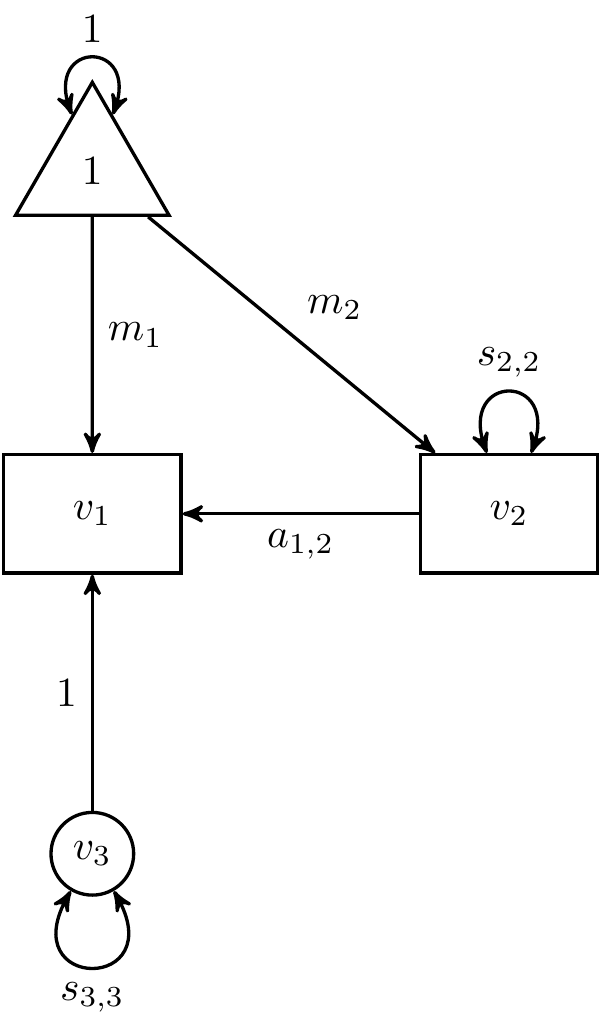
\includegraphics{ram-notes_files/figure-latex/regression-01-1.pdf}
\caption{\label{fig:regression-01}The Simple Linear Regression Model (with \(u\))}
\end{figure}

\hypertarget{expectations}{%
\subsection{Expectations}\label{expectations}}

\begin{equation}
  \mathbb{E}
  \left(
    u
  \right)
  =
  m_3
  =
  0
\end{equation}

\begin{equation}
  \mathbb{E}
  \left(
    v_2
  \right)
  =
  m_2
  =
  13.038328
\end{equation}

\begin{equation}
  \begin{split}
    \mathbb{E}
    \left(
      v_1
    \right)
    &=
    \mathbb{E}
    \left(
      m_1 + a_{1, 2} v_2 + \varepsilon
    \right) \\
    &=
    \mathbb{E}
    \left(
      m_1
    \right)
    +
    \mathbb{E}
    \left(
      a_{1, 2} v_2
    \right)
    +
    \mathbb{E}
    \left(
      \varepsilon
    \right) \\
    &=
    m_1
    +
    a_{1, 2}
    \mathbb{E}
    \left(
      v_2
    \right)
    +
    \mathbb{E}
    \left(
      \varepsilon
    \right) \\
    &=
    m_1
    +
    a_{1, 2}
    m_2
    +
    0 \\
    &=
    m_1
    +
    a_{1, 2}
    m_2 \\
    &=
    -3.951208
    +
    1.269259
    \times
    13.038328 \\
    &=
    12.5978072
  \end{split}
\end{equation}

\begin{equation}
  \begin{split}
    \mathbb{E}
    \left(
      \begin{bmatrix}
        v_1 \\
        v_2 \\
        u
      \end{bmatrix}
    \right)
    &=
    \begin{bmatrix}
      m_1 + a_{1, 2} m_2 \\
      m_2 \\
      m_3
    \end{bmatrix} \\
    &=
    \begin{bmatrix}
      12.5978072 \\
      13.038328 \\
      0
    \end{bmatrix}
  \end{split}
\end{equation}

\begin{equation}
  \begin{split}
    \mathrm{Cov}
    \left(
      u,
      u 
    \right)
    &=
    \mathrm{Var}
    \left(
      u 
    \right) \\
    &=
    \omega_{3, 3} \\
    &=
    47.659854
  \end{split}
\end{equation}

\begin{equation}
  \begin{split}
    \mathrm{Cov}
    \left(
      v_1,
      u 
    \right)
    &=
    \mathrm{Cov}
    \left(
      a_{1, 2} v_2 + u,
      u 
    \right) \\
    &=
    \mathrm{Cov}
    \left(
      a_{1, 2} v_2, u
    \right)
    +
    \mathrm{Cov}
    \left(
      u, u
    \right) \\
    &=
    a_{1, 2}^{2}
    \mathrm{Cov}
    \left(
      v_2, u
    \right)
    +
    \mathrm{Var}
    \left(
      u
    \right) \\
    &=
    a_{1, 2}^{2}
    \cdot
    0
    +
    \omega_{3, 3} \\
    &=
    0
    +
    \omega_{3, 3} \\
    &=
    \omega_{3, 3} \\
    &=
    47.659854
  \end{split}
\end{equation}

\begin{equation}
  \mathrm{Cov}
  \left(
    v_2,
    u 
  \right)
  =
  0
\end{equation}

\begin{equation}
  \begin{split}
    \mathrm{Cov} \left( v_1, v_1 \right)
    &=
    \mathrm{Cov}
    \left(
      a_{1, 2} v_2 + u,
      a_{1, 2} v_2 + u 
    \right) \\
    &=
    \mathrm{Cov} \left( a_{1, 2} v_2, a_{1, 2} v_2 \right)
    +
    \mathrm{Cov} \left( a_{1, 2} v_2, u \right)
    +
    \mathrm{Cov} \left( a_{1, 2} v_2, u \right)
    +
    \mathrm{Cov} \left( u, u \right) \\
    &=
    a_{1, 2}^{2} \mathrm{Cov} \left( v_2 \right)
    +
    a_{1, 2} \mathrm{Cov} \left( v_2, u \right)
    +
    a_{1, 2} \mathrm{Cov} \left( v_2, u \right)
    +
    \mathrm{Var} \left( u, u \right) \\
    &=
    a_{1, 2}^{2} \mathrm{Var} \left( v_2 \right)
    +
    a_{1, 2} 0
    +
    a_{1, 2} 0
    +
    \omega_{3, 3} \\
    &=
    a_{1, 2}^{2} \omega_{2, 2} + \omega_{3, 3} \\
    &=
    1.269259^{2} \times 7.151261 + 47.659854 \\
    &=
    59.1806671
  \end{split}
\end{equation}

\begin{equation}
  \begin{split}
    \mathrm{Cov} \left( v_2, v_1 \right)
    &=
    \mathrm{Cov} \left( v_2, a_{1, 2} v_2 + u \right) \\
    &=
    \mathrm{Cov} \left( v_2, a_{1, 2} v_2 \right)
    +
    \mathrm{Cov} \left( v_2, u \right) \\
    &=
    a_{1, 2} \mathrm{Cov} \left( v_2, v_2 \right)
    +
    0 \\
    &=
    a_{1, 2} \mathrm{Var} \left( v_2 \right) \\
    &=
    a_{1, 2} \omega_{2, 2} \\
    &=
    1.269259 \times 7.151261 \\ 
    &=
    9.0768024 \\ 
  \end{split}
\end{equation}

\begin{equation}
  \begin{split}
    \mathrm{Cov} \left( v_2, v_2 \right)
    &=
    \mathrm{Var} \left( v_2 \right) \\
    &=
    \omega_{2, 2} \\
    &=
    7.151261
  \end{split}
\end{equation}

\begin{equation}
  \begin{split}
    \mathrm{Cov}
    \left(
      \begin{bmatrix}
        v_1 \\
        v_2 \\
        u
      \end{bmatrix}
    \right)
    &=
    \begin{bmatrix}
      a_{1, 2}^{2} \omega_{2, 2} + \omega_{3, 3} & a_{1, 2} \omega_{2, 2} & \omega_{3, 3} \\
      a_{1, 2} \omega_{2, 2} & \omega_{2, 2} & 0 \\
      \omega_{3, 3} & 0 & \omega_{3, 3}
    \end{bmatrix} \\
    &=
    \begin{bmatrix}
      59.1806671 & 9.0768024 & 47.659854 \\
      9.0768024 & 7.151261 & 0 \\
      47.659854 & 0 & 47.659854
    \end{bmatrix}
  \end{split}
\end{equation}

\hypertarget{using-the-ram-package}{%
\subsubsection{\texorpdfstring{Using the \texttt{ram()} Package}{Using the ram() Package}}\label{using-the-ram-package}}

\begin{Shaded}
\begin{Highlighting}[]
\NormalTok{knitr}\SpecialCharTok{::}\FunctionTok{kable}\NormalTok{(}
\NormalTok{  ram}\SpecialCharTok{::}\FunctionTok{mutheta}\NormalTok{(}
\NormalTok{    m,}
    \AttributeTok{A =}\NormalTok{ A,}
    \AttributeTok{filter =}\NormalTok{ filter}
\NormalTok{  ),}
  \AttributeTok{col.names =} \StringTok{"$}\SpecialCharTok{\textbackslash{}\textbackslash{}}\StringTok{boldsymbol\{}\SpecialCharTok{\textbackslash{}\textbackslash{}}\StringTok{mu\}$"}\NormalTok{,}
  \AttributeTok{escape =} \ConstantTok{FALSE}
\NormalTok{)}
\end{Highlighting}
\end{Shaded}

\begin{tabular}{l|r}
\hline
  & $\boldsymbol{\mu}$\\
\hline
$v_1$ & 12.59781\\
\hline
$v_2$ & 13.03833\\
\hline
$u$ & 0.00000\\
\hline
\end{tabular}

\begin{Shaded}
\begin{Highlighting}[]
\NormalTok{knitr}\SpecialCharTok{::}\FunctionTok{kable}\NormalTok{(}
\NormalTok{  ram}\SpecialCharTok{::}\FunctionTok{Sigmatheta}\NormalTok{(}
    \AttributeTok{A =}\NormalTok{ A,}
    \AttributeTok{Omega =}\NormalTok{ Omega,}
    \AttributeTok{filter =}\NormalTok{ filter}
\NormalTok{  ),}
  \AttributeTok{escape =} \ConstantTok{FALSE}
\NormalTok{)}
\end{Highlighting}
\end{Shaded}

\begin{tabular}{l|r|r|r}
\hline
  & $v_1$ & $v_2$ & $u$\\
\hline
$v_1$ & 59.180667 & 9.076802 & 47.65985\\
\hline
$v_2$ & 9.076802 & 7.151261 & 0.00000\\
\hline
$u$ & 47.659854 & 0.000000 & 47.65985\\
\hline
\end{tabular}

\hypertarget{specification-2---observed-variables}{%
\section{Specification 2 - Observed Variables}\label{specification-2---observed-variables}}

\hypertarget{matrix-notation-1}{%
\subsection{Matrix Notation}\label{matrix-notation-1}}

\begin{equation}
  \mathrm{variables}
  =
  \begin{bmatrix}
    v_1 \\
    v_2
  \end{bmatrix}
\end{equation}

\begin{equation}
  \mathbf{A}
  =
  \begin{bmatrix}
    0 & a_{1, 2} \\
    0 & 0
  \end{bmatrix}
  =
  \begin{bmatrix}
    0 & 1.269259 \\
    0 & 0
  \end{bmatrix}
\end{equation}

\begin{equation}
  \boldsymbol{\Omega}
  =
  \begin{bmatrix}
    \omega_{1, 1} & 0             \\
    0             & \omega_{2, 2}
  \end{bmatrix}
  =
  \begin{bmatrix}
    47.659854 & 0 \\
    0 & 7.151261
  \end{bmatrix}
\end{equation}

\begin{equation}
  \mathbf{m}
  =
  \begin{bmatrix}
    m_1 \\
    m_2
  \end{bmatrix}
  =
  \begin{bmatrix}
    -3.951208 \\
    13.038328
  \end{bmatrix}
\end{equation}

\begin{equation}
  \mathbf{F}
  =
  \begin{bmatrix}
    1 & 0 \\
    0 & 1
  \end{bmatrix}
\end{equation}

\hypertarget{path-diagram-1}{%
\subsection{Path Diagram}\label{path-diagram-1}}

\begin{figure}
\centering
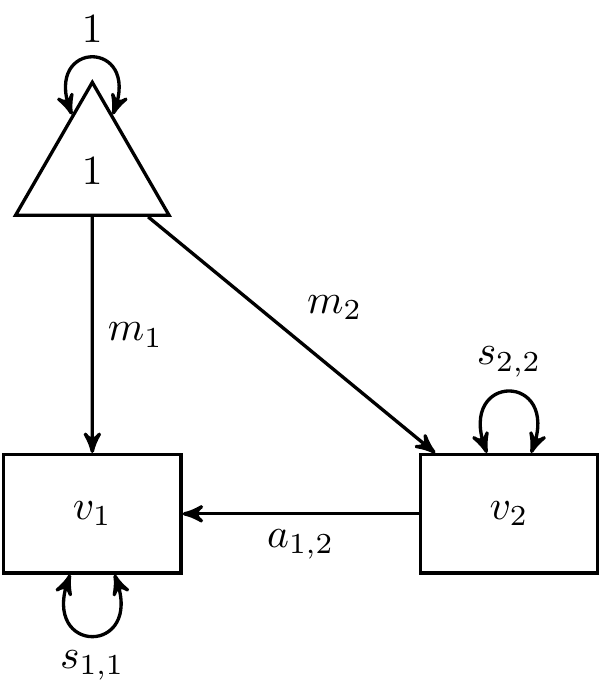
\includegraphics{ram-notes_files/figure-latex/regression-02-1.png}
\caption{\label{fig:regression-02}The Simple Linear Regression Model (without \(u\))}
\end{figure}

\hypertarget{using-the-ram-package-1}{%
\subsubsection{\texorpdfstring{Using the \texttt{ram()} Package}{Using the ram() Package}}\label{using-the-ram-package-1}}

\begin{Shaded}
\begin{Highlighting}[]
\NormalTok{knitr}\SpecialCharTok{::}\FunctionTok{kable}\NormalTok{(}
\NormalTok{  ram}\SpecialCharTok{::}\FunctionTok{mutheta}\NormalTok{(}
\NormalTok{    m,}
    \AttributeTok{A =}\NormalTok{ A,}
    \AttributeTok{filter =}\NormalTok{ filter}
\NormalTok{  ),}
  \AttributeTok{col.names =} \StringTok{"$}\SpecialCharTok{\textbackslash{}\textbackslash{}}\StringTok{boldsymbol\{}\SpecialCharTok{\textbackslash{}\textbackslash{}}\StringTok{mu\}$"}\NormalTok{,}
  \AttributeTok{escape =} \ConstantTok{FALSE}
\NormalTok{)}
\end{Highlighting}
\end{Shaded}

\begin{tabular}{l|r}
\hline
  & $\boldsymbol{\mu}$\\
\hline
$v_1$ & 12.59781\\
\hline
$v_2$ & 13.03833\\
\hline
\end{tabular}

\begin{Shaded}
\begin{Highlighting}[]
\NormalTok{knitr}\SpecialCharTok{::}\FunctionTok{kable}\NormalTok{(}
\NormalTok{  ram}\SpecialCharTok{::}\FunctionTok{Sigmatheta}\NormalTok{(}
    \AttributeTok{A =}\NormalTok{ A,}
    \AttributeTok{Omega =}\NormalTok{ Omega,}
    \AttributeTok{filter =}\NormalTok{ filter}
\NormalTok{  ),}
  \AttributeTok{escape =} \ConstantTok{FALSE}
\NormalTok{)}
\end{Highlighting}
\end{Shaded}

\begin{tabular}{l|r|r}
\hline
  & $v_1$ & $v_2$\\
\hline
$v_1$ & 59.180667 & 9.076802\\
\hline
$v_2$ & 9.076802 & 7.151261\\
\hline
\end{tabular}

  \bibliography{book.bib,packages.bib}

\end{document}
